\chapter{Analysis \& Design of the Solution}
\label{analysis_design}

The purpose of Metadata Extractor is to obtain metadata from data models that were created using modeling tools ER/Studio and PowerDesigner. 
The solution will be able to interact with Manta Flow and bring business lineage on objects from physical and logical data models. 
Currently, Manta Flow supports only automated creation of technical lineage.

Here we describe how we proceeded when analyzing the solution and discuss crucial features of ER/Studio and PowerDesigner in detail.
Therefore, we can identify the important aspects of the tool that we will need to focus on, when finally implementing Metadata Extractor.\\

In this chapter we seek answers for these questions:
\begin{enumerate}
	\item Identify what data models the modeling tools work with, what objects are contained in the supported data models, how they are organized and what metadata can be obtained that are relevant to be brought into data lineage.
	\item Find out how the data models are saved and how the interesting information from 1) can be reconstructed.
	\item Determine how the file format in what data models are stored can be parsed.
\end{enumerate}

\section{Analysis of the Problem}

We already presented that the modeling tools are capable of creating data models. These models are saved into files. 
The output files of the modeling tools are going to be the input of Metadata Extractor, that uses them for reconstruction of the objects and information contained in the data models.
In order to come with logic of the reconstruction, we need to identify what objects are saved in the files produced by modeling tools, and how they are represented. 
In \Cref{chap:database_modeling} about database modeling we introduced the standard layout of every data model type. We will quickly review their main objects. \\

\label{main_modeled_objects}
Conceptual and logical data models consist of entities, which may have attributes.
Physical data models are made of tables. A table is composed of columns may belong to a schema.

These are the fundamental metadata Metadata Extractor must load form the files. 
Consequently, it must correctly load hierarchy of these objects as it is modeled. For example attributes must be assigned to entities correctly, etc.

Next, we will look at how to find the pairs of objects that are in maps-to relation, and how do they refer to each other across levels of abstraction.
In example, how a logical attribute and a physical column, are tied together across data models.

\subsection{File Format}

In this section we firstly discuss what is the output of the analyzed modeling tools. Then we look at the main principles of how and what information is stored in the given format. Knowing this Metadata Extractor we can find the required objects (mentioned in \Cref{main_modeled_objects}) serialized in a file.

\subsubsection{ER/Studio}
\label{subsec:dm1_format}

The ER/Studio modeling tool uses its custom file format. These files have the .DM1 extension. 
In a single .DM1 file, related data models are stored. Let's call these models a solution. An \definition{ER/Studio solution} is set of data models, describing a problem on both logical and physical levels (the two layers are only that ER/Studio supports). 
In a solution one logical model must be present whereas 0 to N physical ones supporting the logical model.
We can imagine why ER/Studio behaves like this. The motivation may be, that once there is a problem (if there is no challenge, no data modeling is needed), must be described by a logical model. 
Possibly user has worked out the way to solve it, and that is when physical models are present as well.
Note that the actual storage may be distributed and the corresponding databases can be of different technologies, that is why more than one physical model is allowed in a single solution.

.DM1 is a textual file format which is organized into many tables.
Such table is a CSV (comma-separated values) structure with a modification, since the file format consists of many of these tables, (i) each table has a unique name which identifies it. 
Next, (ii) a table contains a CSV row, which defines each column of the table. 
Lastly, (iii) CSV rows are standing for records that are stored in a table. 
To put it together, by a single table in .DM1 file we understand its name, column definitions and records (rows representing data stored in the table).
At the first sight, it is not clear how complex objects can be stored in files that we just described. To get the idea behind it, we did some work that we are going to described in this section. 

\begin{figure}[H]
	\centering
	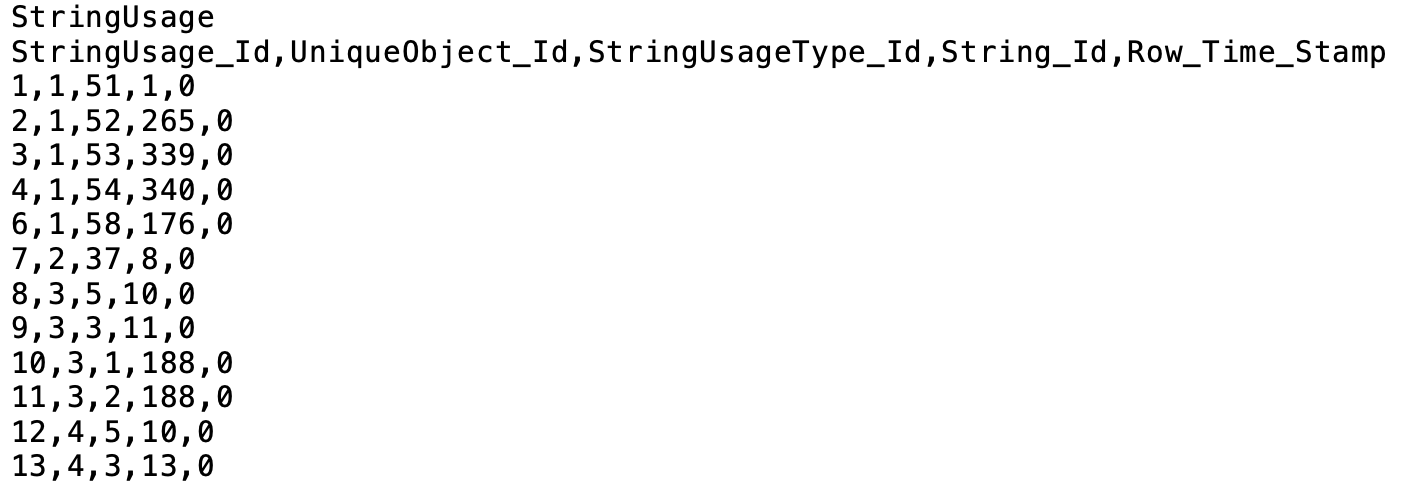
\includegraphics[width=14cm]{../img/StringUsageTable}
	\caption[Table from .DM1 file]{Example of a simple CSV table from a .DM1 file. It is named StringUsage, is made of five columns and stores 13 records.}
\end{figure}


An attentive reader may find the terms we used for when describing a .DM1 table familiar. 
As we already seen the terminology when introducing relational databases (see \Cref{relational_databases}). 
When going through the tables, we can notice columns that have common names.
That resembles primary and foreign key concepts used in relational databases, where a column is used to reference a record stored a different table. 
The keys indicate relations between tables.

It looks like this could be the answer for the question we proposed earlier - how complex objects can be stored in the simple tables. Each table stores a simple aspect of an object, but thanks to the relations, interconnected tables can linked together and compose from their data a more complicated object.

To identify crucial relations, that Metadata Extractor needs to know, in order to be able to reconstruct composite objects such as entities, attributes, etc., from .DM1 files, we developed a little reverse-engineering utility, which helps us to get an overview of the links between the tables.
Further details on how we proceeded when designing the utility can be found in \Cref{subsec:dm1_tool}. 

In order to work with a .DM1 file programmatically, it is needed to load it into suitable data structures, that can be processed further. That is what a parser does. 
Metadata Extractor, as well as the reverse-engineering utility need such parser.
We mentioned the file format is basically a sequence of CSV tables. 
The question was whether to reach out for an existing CSV parsing solution, or to develop a tailor made one.
We took the second option, why and how we did so is described further in \Cref{subsec:dm1_parser}. \\

To sum up, the reverse-engineering utility provides an insight into the logic of .DM1 files, so Metadata Extractor knows what data model objects are stored in the files and how the complex objects are deserialized there. The parser prepares an input file, thus Metadata Extractor can reconstruct the objects and their metadata stored in it.

\subsubsection{PowerDesigner}

PowerDesigner produces files storing data models with three types of extensions - .pdm, .ldm and .cdm.
They stand for physical, logical and conceptual data model respectively.

While ER/Studio groups data models into solutions every model created in PowerDesigner is saved independently. 
A set of files that are at the same time opened in PowerDesigner forms its state. 
Such state is called a workspace and can be saved into a .sws file. However, the workspace files do not bring us anything interesting. 
The information captured stores only what data models were at some time opened in user's interface and does not tell anything about logical links between the files.

The data model files are XML (Extensible Markup Language) based file formats.
Alternatively, PowerDesigner is also able to save its data models into a binary file. The advantage is that the binary files can be processed more quickly and are smaller in size than the XML counterparts. 
However, we need a Metadata Extractor user to save his models as XMLs, that is the only this way currently supported.

When parsing XML files there are two major ways how to do it. \\

The first approach is SAX (Simple API for XML), which is an event-driven parser that process an XML document sequentially by a single pass. 
By default its processing is stateless and handlers are triggered when an event occurs. 
It is a simple and lightweight XML parser. \\

On the other hand, we have a family of DOM (Document Object Model) parsers. 
They load an XML file into a full AST (Abstract Syntactic Tree) structure. 
This way of file processing more memory and time consuming, but translates everything stored in the input file into data structure straightforwardly. 
Then it can be conveniently worked with the tree-like resulting structure, where nodes represent parts of the processed document. \\

The great aspect of XML files is that they are human-readable and to figure out how the objects, Metadata Extractor is seeking for, are serialized in these files is not that difficult.
In the next section we describe what objects and information Metadata Extractor has to retrieve from the PowerDesigner data model files. We will see that the objects and their properties are quite complex.
Having a stateful parser would bring an advantage as the context of the XML elements matter, since, for example a definition, Metadata Extractor has to obtain, can be attached to an entity, an attribute and many other kinds of objects.
Therefore, using a DOM parser is much more suitable and having the ability of doing XPath queries over a DOM document is nicer than having to store a context manually, what would be needed to do with SAX.

\subsection{Metadata to Collect from Data Models}
\label{metadata_enumeration}

The main goal of Metadata Extractor is to bring business data lineage and to extract metadata for objects in both business data lineage and the technical one.
To meet the goal, we have to identify what objects and which of their metadata to collect from data models on every level of abstraction.

Metadata Extractor is aimed to bring information that is relevant to for data lineage and may be visualized when presenting a flow of data.
Modeling tools are exhaustive pieces of software with many features, thus have the ability to capture plenty of aspects that a modeled system has.
We determined types information, that can appear in data models of PowerDesigner and ER/Studio, makes sense to extract by analysis. Let us mention two important categories of metadata that we assume irrelevant to retrieve by Metadata Extractor.

Firstly, we will not pay attention to relationships in the entity-relationship model. 
This is given by the nature of Manta Flow. It is not a modeling tool, thus it does not work with relations and edges between objects are used solely to represent flow of data in a given system.
The only relationship type from data models we will need to cope with is the inheritance relation, which is present in the enhanced-entity-relationship model. 
The difference is that without capturing the is-a links, an entity may not be described completely and the attributes that are inherited may be missing.

The second category of metadata that Metadata Extractor will ignore, are the ones that describe constraints on the actual data records saved in a database. 
Metadata Extractor works, just like Manta Flow, exclusively with database's metadata and does not access the data really saved in a storage. 
Thus, our solution neither can monitor nor enforce any constraint on the database entries. 
That is why the metadata like keys or data types, which are also defined in data models, will not be in our domain of interest.

In this section we list the specific types of objects we considered important for data lineage and what are the means to describe these objects even further by properties of theirs. 
The full list of metadata, including the ones we do not find useful to extract, is listed in \Cref{full_list_metadata}.

\subsubsection{Conceptual \& Logical Data Model}

Here we go through objects that appear in both conceptual and logical data models, together with what additional metadata can be attached to them.

\subsubsection{ER/Studio}

\subsubsection{CDM}

ER/Studio Data Architect does not support conceptual data models.

\subsubsection{LDM}

\begin{itemize}
	\item Owner \\ 
	An owner is a concept equivalent to a schema - it is a container for logically related entities. Every entity belongs to an owner.
	\item Entity \\
	\begin{itemize}
		\item Name \\ 
		The name of an entity.
		\item Attributes \\ 
		Attributes assigned to an entity.
		\item Definition \\
		Further description of an entity. Plain text or RTF (rich text format).
		\item Note \\
		Notes are used when a documentation about an entity is generated. Plain text or RTF.
		\item Where Used \\
		This property shows objects that are in maps-to relation with an entity. Those which were created by generating.
		\item User-Defined Mappings \\
		Shows objects that are in maps-to relation with an entity. These mapping are user defined. They can contain description of a relation, but we will not fetch the text as Manta Flow does not support attributes on mapping edges.
		\item Owner \\ 
		The owner an entity belongs to.
	\end{itemize}
	\item Attribute
	\begin{itemize}
		\item Name
		\item Definition
		\item Notes
		\item Where Used
		\item User-Defined Mappings
	\end{itemize}
\end{itemize}


\subsubsection{PowerDesigner}

Conceptual and logical data models in PowerDesigner have so much in common that we will propose unified view on what may be stored in them. The properties/object that are specific for either of them are marked with information in brackets saying "CDM/LDM only".

\subsubsection{CDM \& LDM}

\begin{itemize}
	\item Data Item (CDM only) \\
	A data item holds an elementary piece of information, which is given by some fact or a definition in a modeled system. It may or may not be present as a modeled object. Data items can be attached to entities to form their attributes. It is a datum that may seem relevant and is possible to capture at first but later may be not used as no entity needs it in the end.
	\begin{itemize}
		\item Name
		\item Code
		\item Comment \\
		Plain text short description.
		\item Definition \\
		An RTF description of an object.
		\item Annotation
		A further RTF description.
		\item Keywords
		Set of significant words specifying object's domain.
	\end{itemize}
	\item Entities
	\begin{itemize}
		\item Name 
		\item Attributes
		\item Code 
		\item Comment
		\item Definition
		\item Annotation
		\item Keywords
	\end{itemize}
	\item Attributes
	\begin{itemize}
		\item Name 
		\item Code 
		\item Comment
		\item Definition
		\item Annotation
		\item Keywords
		\item Parent Entity
	\end{itemize}
	\item Inheritances
	\begin{itemize}
		\item Parent Entity \\ 
		Predecessor.
		\item Child Entity \\ 
		Inheriting entity that takes over attributes of the parent.
	\end{itemize}
\end{itemize}

\subsubsection{Physical Data Model}

In this section we list objects from physical level and their possible metadata.

\subsubsection{ER/Studio}

\begin{itemize}
	\item Type of Data Model\\
	Database management system that a model is aimed for.
	\item Schema
	 \begin{itemize}
	 	\item Name
	 	\item Tables
	 \end{itemize}
	\item Table
	\begin{itemize}
		\item Name
		\item Columns
		\item Schema
		\item Definition
		\item Note
		\item Where Used
		\item User-Defined Mappings
	\end{itemize}
	\item Column
	\begin{itemize}
		\item Name
		\item Definition
		\item Notes
		\item Where Used
		\item User-Defined Mappings
	\end{itemize}
\end{itemize}

\subsubsection{PowerDesigner}

\begin{itemize}
	\item Tables
	\begin{itemize}
		\item Name 
		\item Columns
		\item Code 
		\item Comment
		\item Definition
		\item Annotation
		\item Keywords
		\item Schema
	\end{itemize}
	\item Columns
	\begin{itemize}
		\item Name 
		\item Code 
		\item Comment
		\item Definition
		\item Annotation
		\item Keywords
		\item Table
	\end{itemize}
\end{itemize}

\subsection{Reconstruction of Data Model}

Earlier in \Cref{metadata_enumeration} we defined what are the objects and their properties that Metadata Extractor must obtain from data models.
The objects living in the common environment of a data model, are related to each other into some kind of hierarchy.
The listing of the objects with their characteristics, which Metadata Extractor will retrieve from data models, makes us realize, that the very basic layout of objects captured by a model resembles a tree-like structure.
The reason is that the analysis implies a general skeleton of a data model that goes like shown in \Cref{DataModelHierarchy}. However, it is just a simplified view. For example, data models do not need to support the concept of owners/schemas.

\begin{figure}[H]
	\centering
	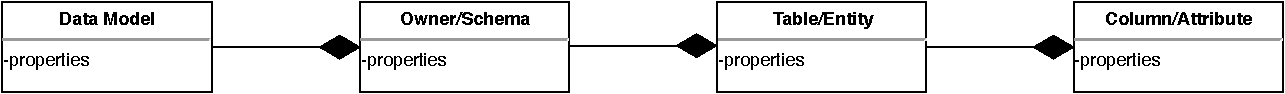
\includegraphics[width=14cm]{../img/DataModelHierarchy}
	\caption[Hierarchy of Objects in a Data Model]{General hierarchy of objects in a data model. The UML diagram pictures a data model, that contains arbitrary number of owners (schemas respectively), they own 0 to N tables (entities resp.), while each entity consists of zero or more columns (attributes resp.). These objects can be seen as nodes of a tree, whereas their properties are attributes of the corresponding nodes.}
	\label{DataModelHierarchy}
\end{figure} 

Surely further relations between the objects will come to play, like inheritances or mappings. They are going to be discussed later in the \Cref{maps_to_analysis}, making the diagram of objects in a data model more complex.
 
Metadata Extractor builds the tree from the top to the bottom. 
In the next two subsections we will describe how the main objects from \Cref{DataModelHierarchy} can be reconstructed from the output files of ER/Studio, PowerDesigner respectively.

\subsubsection{ER/Studio}

In the case of ER/Studio, each type of the objects is defined in a single table. Such table stores all instances of the given type. 
An instance is identified in a table uniquely by its ID among other realizations of the same type.
Therefore, this ID is a primary key of a table. The relations from \Cref{DataModelHierarchy} are 
done by these keys.
An object has a reference to its, if we stick with the tree terminology, parent by storing parent's ID as a foreign key property of itself. 
Object's textual properties like name or definition are saved in a table containing string entries. 
Tables storing the records of the main objects therefore have also column with foreign keys to the string table. 
So if Metadata Extractor proceeds by loading data models firstly, then descending down the tree, every time it is loading an object, its parent has already been constructed and the child can be simply plugged to the parent that the child references by a foreign key.

\subsubsection{PowerDesigner}

XML files form a tree structure by definition. This fact makes storing a hierarchy of objects with the same nature suitable and straightforward. 
This way a parent object of a child is simply its predecessor in the tree formed by XML elements of a file. 
Properties of an object are stored as child XML elements.
When Metadata Extractor creates the result, the top-down traversal of an XML tree is followed. 
At first, on its way down from the XML root, it builds objects higher in the hierarchy and only if a parent is build, Extractor examines its children. 
This way the context is clear and once, let's say an attribute, is created the program knows what is its parent entity trivially, as it must be the one that was created most recently.

\subsection{Maps-to Relation}
\label{maps_to_analysis}

Once we identified possible objects across the data models, it is really useful to know which objects are related, even though they were not defined at the same level of abstraction. 
It is important to keep the data models readable, and to keep track of what tables are implementing which high level concept.

Our tool deals only with mappings of objects which are not at the same level of abstraction. 
Some modeling tools allow mapping, for example, a logical entity to a logical but it is unclear what is the meaning of such construct. 
One explanation would be, that it expresses a relationship, but data modeling tools have other means available for defining relationships. 
Possibly, it could indicate that the entities are used identically as they are implemented by a single database table, but that is what data lineage describes precisely and will be brought by Metadata Extractor.

To be specific Metadata Extractor copes only with the following types mappings: 
\begin{itemize}
	\item An entity to a table or another entity. 
	\item An attribute to a column or another attribute.
\end{itemize}
\label{allowed_mappings}

Now we take a look how the mapping are realized in the chosen data modeling tools.

\subsubsection{ER/Studio}

In \Cref{metadata_enumeration} we mentioned two types of mapping relations in ER/Studio for  entities, tables, attributes and columns.
In fact, meaning of both types is the same. The only difference is that the where-used mappings are generated automatically, while the user-defined are drawn manually by a user. 
We assumed that all the objects that can appear in maps-to relation are in the very same solution, but there is also an option to create a mapping to objects which are defined in different .DM1 files. It can be done using the Compare and Merge utility in ER/Studio, whose functionality is to synchronize a model with another model/live database/SQL file. 
Among other operations that keep pairs in sync, there is the mapping creation option. 
We are interested in the first scenario, where the two compared data models may originate even in two different solutions. 
This, third, kind of maps-to relation is referred to as a universal mapping. \\

Knowing all the possible types of the mapping relation, we will further focus on how they are saved in an ER/Studio .DM1 file and how can they be extracted. \\ 

Let's start with the seemingly easier case of mappings between objects inside the same ER/Studio solution - where-used and user-defined. 
After some analysis using the reverse-engineering tools (see \Cref{data_model_reverse_engineering}) we found the table that stores the mappings. It is named Where\textunderscore Used\textunderscore PD.
In the table, there are four crucial attributes, IDs of the mapped objects and their Meta table types.
The first two attributes are foreign keys to tables, where the mapped objects are defined. The second pair of columns defines a type of the object, so that Metadata Extractor knows to which tables it should look for the instances that are referenced by the foreign keys. 
The Meta table types also allows us to check, if the objects are actually compatible with each other in the sense of how we constrained the allowed mappings in \Cref{allowed_mappings}. \\

At the first sight, solving the universal mappings may appear more difficult. It looks like Metadata Extractor will need to search for object in different ER/Studio solutions and reconstruct the external objects. 
But the way the universal mappings are realized in ER/Studio is much simpler. 
Metadata Extractor does not need to open other files, as the external objects that are referenced by a universal mapping are stored in the analyzed .DM1 file. 
They are described briefly in a table called External\textunderscore Mapped\textunderscore Objects by XML structures.
Metadata Extractor uses SAX parser to load these objects, as the XML object description is simple.
Finally, the table called Universal\textunderscore Mappings, where the all the mappings to external objects are defined, is using the same concepts as Where\textunderscore Used\textunderscore PD allowing Metadata Extractor to reconstruct them easily.

\subsubsection{PowerDesigner}

PowerDesigner saves every data model into a separate file. Therefore, to resolve mappings will be not as straightforward as in the case of ER/Studio, since every mapping of an object to another that is on a different abstraction layer leads across PowerDesigner files.
Firstly, let's go through the possible types of mappings, then we will discuss how to resolve the relation efficiently.

The mappings are divided into two categories. 
Similarly as in the first tool, the mappings may be either generated or user-defined. \\ 


Before going through how the mappings are represented, we must mention the way objects taking part in the relation are identified.
Every important objects in PowerDesigner has a unique identifier named ObjectID. This sequence of characters is used when referring to the object.\\

When an object is created out of an existing one by generating, the resulting object has an XML element named History. The element contains holds all the IDs of objects that the final object was generated from.

User defined mappings are represented by a composite XML element. 
The element representing a single mapping consists of a pair of mapped entities/tables IDs. If sub objects of the pair are tied together by mapping as well, the XML element is a parent of further XML elements, which are specifying IDs of the underlying attributes/columns that are mapped to each other. \\

However, knowing the types of mappings and how they are saved in the PowerDesigner files is not enough to reconstruct the relation. Let's imagine the following scenario.
Metadata Extractor gets a file to process. It reconstructs objects stored in the file, then the program tries to resolve mappings, but one of the mapped objects is not accessible, as it is defined in a different file, than is the one Metadata Extractor is currently reading.
Only the ID of the mapped counterpart is known. 
In order to gather all the required metadata about the mapped object, Metadata Extractor needs to find it by its ID in the file where it is defined.
Thus in a situation like this, data model file are dependent on others.
In PowerDesigner's file format Metadata Extractor can find an XML element describing targets of the given model, to learn what are the files it depends on.

When a model is generated from a file, such dependency is saved to both of the data model files, in the generation target as well as in the origin. 
In other words, if we imagine an oriented graph, where a file is a node and an edge leads from a file $a$ to file $b$ $\iff$ $b$ is listed as a dependency of $a$, then bidirectional edge is created when models are generated.

Whereas, when a user-defined mapping is created from an object in a source model $c$ to an object in a target model $d$, only the $c \rightarrow d$ edge is created, and $d$ has no knowledge about the mapping.
Metadata Extractor must solve how a resolution of the external objects will be done. 
As it has no further knowledge than the target object's ID, not even information what file does it come from, a naïve approach would be hugely inefficient. 
The simple solution would search for every demanded ID across all targets of the processed model and once the ID is found, the objects gets reconstructed. 
That potentially leads to a great amount of file openings. Also if an object is referenced from $n$ mappings, it would have to be reconstructed $n$ times while still processing a single data model, leading to a huge time overhead.
Surely, this solution can be improved by collecting the external IDs and postponing the resolution to the end, once all the needed external objects are known. 
So when processing a single file, each of its target would be opened only once and the reconstruction of the object would take place one time as well. But still, if an object is referenced from $n$ different models, it would be reconstructed $n + 1$ times, which definitely not ideal.

If we went in a different direction and processed each of the model once, constructed all their objects, then stored all of them by their IDs and once all the data models that Metadata Extractor had to process are loaded, resolve mappings. 
Advancing like this would decreased count of reconstructions and file openings to the ideal amount but eventually, if the number of inputted data models is big the size of memory claimed by Metadata Extractor could become unbearable.

To achieve a solution that would have the advantages of both of the approaches, Metadata Extractor needs to split the set of input models into disjoint subsets, that represent the smallest group of logically tied files. 
Metadata Extractor transforms all of the unidirectional edges in the dependency graph described above (and illustrated in \Cref{PDComponents}), into bidirectional and finds connected components. These components are the logical subsets. 
Therefore the program can reconstruct objects from a single component and make the resolution at the end. That keeps the storage acquired by loaded objects low and at the same time objects are constructed only once, while files don't get opened multiple times. 
We assume, that the far most common use-case is having components of size three with three data models - logical, conceptual and physical (or few physical ones). \\

\begin{figure}[H]
	\centering
	\begin{center}
		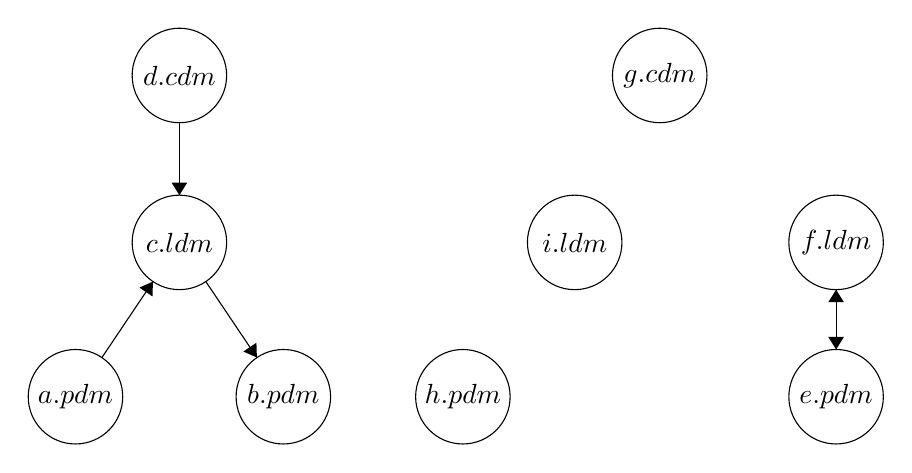
\begin{tikzpicture}[scale=0.2]
		\tikzstyle{every node}+=[inner sep=0pt]
		\draw [black] (7.9,-32.9) circle (3);
		\draw (7.9,-32.9) node {$a.pdm$};
		\draw [black] (21.1,-32.9) circle (3);
		\draw (21.1,-32.9) node {$b.pdm$};
		\draw [black] (14.5,-23.1) circle (3);
		\draw (14.5,-23.1) node {$c.ldm$};
		\draw [black] (14.5,-12.5) circle (3);
		\draw (14.5,-12.5) node {$d.cdm$};
		\draw [black] (56.2,-32.9) circle (3);
		\draw (56.2,-32.9) node {$e.pdm$};
		\draw [black] (56.2,-23.1) circle (3);
		\draw (56.2,-23.1) node {$f.ldm$};
		\draw [black] (45,-12.5) circle (3);
		\draw (45,-12.5) node {$g.cdm$};
		\draw [black] (32.5,-32.9) circle (3);
		\draw (32.5,-32.9) node {$h.pdm$};
		\draw [black] (39.6,-23.1) circle (3);
		\draw (39.6,-23.1) node {$i.ldm$};
		\draw [black] (9.58,-30.41) -- (12.82,-25.59);
		\fill [black] (12.82,-25.59) -- (11.96,-25.97) -- (12.79,-26.53);
		\draw [black] (16.18,-25.59) -- (19.42,-30.41);
		\fill [black] (19.42,-30.41) -- (19.39,-29.47) -- (18.56,-30.03);
		\draw [black] (14.5,-15.5) -- (14.5,-20.1);
		\fill [black] (14.5,-20.1) -- (15,-19.3) -- (14,-19.3);
		\draw [black] (56.2,-26.1) -- (56.2,-29.9);
		\fill [black] (56.2,-29.9) -- (56.7,-29.1) -- (55.7,-29.1);
		\draw [black] (56.2,-29.9) -- (56.2,-26.1);
		\fill [black] (56.2,-26.1) -- (55.7,-26.9) -- (56.7,-26.9);
		\end{tikzpicture}
	\end{center}
	\caption[PowerDesigner Components Example]{On the example we have four five  components made of PowerDesigner data models. If dependencies of data models are like this, a.pdm should get processed and resolved in one batch with b.pdm, c.ldm and d.cdm. Then f.ldm must be handled with e.pdm, while rest of the models are independent and form component of size one.}
	\label{PDComponents}
\end{figure}

However, when dealing with the dependencies, there is one more trap remaining that may cause problems. The basic scenario how a user behaves when using Metadata Extractor is that he works with PowerDesigner data models that are saved somewhere, for example in C:/PowerDesigner/Project/, and once he wants to let them analyze by Metadata Extractor, he drags them to a different directory, that is used as input for our tool.
This way, paths pointing to target models become incorrect, since the paths don't get updated until the moved files are not opened again. 
So the models in input still depend on files in C:/PowerDesigner/Project/ which may be not existing anymore. Alternatively, if the paths remain incorrect there may happen a situation like this - we have a file $a$ referring to $b$ in, both of them in input, but a change of an object in C:/PowerDesigner/Project/$b$ affects $a$ that is using the changed object due to the described problem.
Anyway, we want Metadata Extractor to work only with the files that a user explicitly marked as to process, those are the ones present in the input directory.
So Metadata Extractor has to have a fallback for this situation and should try to find target files in input folder.
The idea is to try the ideal scenario and check whether the target is in the input directory. If yes, the resolution is done.
Otherwise the program assumes a similar structure of the former and input directory, as well as that names of data model files did not changed.

\subsection{Business Lineage Creation}

One of the main goals of this work is to develop make Metadata Extractor capable of creating business\footnote{By business lineage we mean data lineage that is formed on a higher level on abstraction than on the physical level.} data lineage automatically.
The way we chose to approach the problem is that Metadata Extractor builds the high-level lineage based on the technical one created by Manta Flow. 
The physical lineage provides the most precise foundation possible. 
It is directly aligned with how a live database system is really used and how data travels through it.
Despite the fact that Manta Flow primarily focuses on analysis of physical data flow, there is an already implemented functionality, which can propagate lineage from physical objects via mapping edges to objects on higher levels of abstraction.
The process of propagating the data flow acquired on physical level to logical or conceptual level is called \definition{interpolation}.
The crucial part is to ensure that Metadata Extractor merges correctly physical modeled objects with their database counterparts that are used by Manta Flow.

\subsection{Database Connections}

Even though Metadata Extractor will not connect to databases directly, it needs to gain details of a database connections when working with physical models.
Only then Metadata Extractor is able to know what specific database the extracted physical objects belong to. Firstly, we will go through why do we actually need the connections and then we will look at how in case of PowerDesigner and ER/Studio the connection can be made and obtained.

What we will do is not accessing metastores \footnote{Shortly for metadata storage} of databases. Getting metadata directly is not really straightforward as each database technology has its own specifics - types of metadata and their organization varies greatly. 
Instead we will make use of the fact that Manta does has connectors that do the job for us, stores the metadata in its own local database and has unified API for getting the metadata independently of database engine. 

And why would we want to request another metadata when that is just what we are extracting from physical data models? \label{matching_physical_objects}
Because we are interested in data lineage, which is created by Manta Flow based on the real metadata of physical objects that are present in a database.
The simple view is that at the moment, when we ask for the objects from Manta Flow's metastore, the analysis of data flow has already taken part, thus there are data lineage edges between physical objects. To bring together both features of Manta Flow and Metadata Extractor, the program must merge equivalent physical objects which come from the both sources - from Manta's extraction and from our tool.
Thus, only if Metadata Extractor is on the same page with Manta Flow - knows what specific database at what specific server the modeled objects belong to, the program can ensure correct pairing of the objects and data lineage. \\

The details we use for identification of a database instance are the following:
\begin{itemize}
	\item Database Type (Technology)
	\item Database Name
	\item Server Name
	\item Schema Name
	\item User Name
\end{itemize} 
All the above can be stored in one property called \definition{connection string}.\\
To this set of the listed properties and a connection string we will refer as a \definition{connection}. \\
Since each physical data model describes a single database (or its subset) we need exactly one connection for each processed physical model in order to achieve what we described just above.

However, the identification of a database that a physical data model reflects cannot be found in the file storing the physical model, we have to inspect other possibilities for to obtaining the database details.

\subsubsection{ER/Studio}

Databases whose models are created in ER/Studio can be reached only by ODBC drivers present in the used machine.

Metadata Extractor is not able to reach these drivers generally, so we will leave it up to a user to define connection parameters by hand.
A .ini files \label{ini_connections}is used for that where sections are named by physical models that they correspond to and connection details are specified inside a section. 

Metadata Extractor tries to get as much information as possible from an ER/Studio data model, however name of a database and server must be added manually by a user as the tool does not save these data.

\subsubsection{PowerDesigner}

In PowerDesigner a user has multiple options for connecting to a database to choose from. Either ODBC or JDBC connection may be used. 
The tool has a nice user environment for creating or using connections to a database where a user is guided through a set up and can test if he did set up everything correctly. 
There are two options of how to connect to a database using the interface that may be helpful for Metadata Extractor, using .dsn and .dcp files.\\

The .dsn files are definitions of ODBC connection containing parameters for an ODBC driver and stores all the interesting information we would like to have. 
The drawback of this file format is that it varies from a database technology to database technology - the properties representing the same concepts may be called differently. That means we would need to have a parser for each supported database engine. \\

On the other hand there is possibility of connecting via .dcp files. They can store information about a native DBMS connection or about a JDBC connection. 
The nice fact about them is that they are not that flexible and once we know whether we deal with a native or a JDBC connection respectively, the structure can be parsed easily. 
The file consisting of property=value map.
There are couple of properties common for both types, like description and user name.
Then the most important property of a JDBC .dcp file is the JDBC connection URL - in other words a connection string which sufficiently defines a connection.
In case of the native DBMS variant, Server Name along with Database Name are crucial, in order to identify a database we are connecting to by the setup.

But there is a problem that is common for both of the approaches -  there is no link between the connection file and a model that corresponds to the connection. 
So Metadata Extractor has to stick with the same solution as in the case of ER/Studio - to use auxiliary .ini files. \Cref{ini_connections}.

\subsection{Output Representation}

The output of Metadata Extractor is a graph. Its nodes are the important extracted objects such as entity, attribute, etc. properties of the nodes will be the metadata acquired about the extracted objects. Edges of the output graph are of different types, they can either stand for mapping of the nodes of indicate flow of data between them. 
The remaining part is how we will represent the output. We require a structure that is both convenient to work with programmatically as a data structure and able to be visually presented to a user of our tool.
Also, we must take into account that Metadata Extractor is going to be plugged into an already existing software environment. 
Manta Flow is backed by a database storing graphs of data lineage. There is already an existing browser-based user interface, using which the data flows can be shown and previewed interactively. 
Given that we would like to comply with the graph database and merge our graphs to the storage, and having the ability to reuse the visualization for presentation of the outputs, the most natural solution is to stick with the very same representation of graph as Manta does.
In the alternative scenario when we don't want to let Manta handle the output, there is a possibility of using a writer which produces an image, or a textual representation of the output at a local machine, in contrary to sending the output to the Manta Server where the graph database is located.

\section{Desired Features}

The analysis forms a set of functional requirements or features we expect Metadata Extractor to have:

\begin{itemize}
	\item Load objects and their metadata from output of modeling tools and reconstruct hierarchy of the objects.
	\begin{itemize}
		\item ER/Studio: Logical data model \& physical data model.
		\item PowerDesigner:  Conceptual data model, logical data model \& physical data model.
	\end{itemize}
	\item Resolve mappings leading between objects originating in different data models.
	\item For every physical data models, obtain connection details to the database counterpart.
	\item Match the loaded physical objects with their equivalents extracted by Manta Flow if possible, in order to bring in the physical data lineage they take part in, so the business lineage can be interpolated.
	\item Create a graph out of the loaded structure. \\
	So that it can be further:
	\begin{itemize}
		\item Displayed in the user interface of Manta.
		\item Printed to a file as image.
	\end{itemize}
\end{itemize}


\section{Survey of Existing Solutions}

We are working on development of an automated solution that delivers business lineage.
In order to justify, that we are not reinventing a wheel let's have a look at the software can provide similar functionality as Metadata Extractor.

The competitors can be divided into multiple categories:

\begin{itemize}
	\item Data Governance Frameworks \\ 
	\definition{Data governance} is a discipline that helps enterprises to gain control over their data. Commonly data lineage is a part of functionality that data governance solutions provide. \\
	Usually the solutions work with \definition{business glossary} which is a set of terms used in business together with their definitions specifying what they precisely mean in a domain. It unifies a vocabulary between system's stakeholders to avoid misinterpretations when it comes to high-level terms. 
	\begin{itemize}
		\item Collibra \\ 
		Works with business assets that connects business terms from glossary to data assets (eg. database column or table). The connections are established manually\cite{CollibraBusinessAssets}. In data lineage diagram business terms can be displayed along with the related data assets to ensure better traceability\cite{CollibraVisualization}.
		\item Informatica Axon \& EDC \\ 
		The solution by Informatica Corporation works on a very similar base as the previous one.
		Data assets are connected by hand in a user interface to business glossary entries\cite{InformaticaBusinessAssets}. That allows, once a technical data lineage is created, to drill down to the data lineage going thorough the mapped database elements. In the data flow can be also found related business assets next to related tables.
		\item IBM IGC \\ 
		IBM approaches to data lineage in such way that it only displays assets that should be relevant for a business user. In fact it is just a subset of technical lineage and what is shown is picked by a user \cite{IbmIgcBusinessLineage}.
	\end{itemize}
	\item Data Lineage Tools \\ 
		A data lineage company asg technologies company seem to do something with modeling tools as they apparently dispose of connectors for some modeling software. However no appropriate documentation can be found and the latest update traceable on ER/Studio connector was made in early 2014. \cite{AsgErStudio}
		The supported version of ER/Studio is 9.7, while the version 18.0 is out today.
		Similarly with their PowerDesigner connector, it is not easy to find a documentation and even if something related is mentioned the information seem to be obsolete nowadays.
	
	\item Modeling tools \\
	Both of the analyzed tools, ER/Studio and PowerDesigner, have means to create something like data lineage models, or lineage can be specified by mappings in a single data model. The problem with this approach is that it is not based on an analysis of SQL code managing the database and the approach is not automated. Creating such models is exhaustive and error prone as a user has to define the flow all by himself. 
\end{itemize}


To our knowledge none of the solutions disposes of the automated functionality we aim to provide by putting together Modeling Tools, Manta Flow and finally Metadata Extractor. That is to create an abstraction over technical details of databases, summarizing the real data flow using business vocabulary.

\section{Architecture of the System}

Metadata Extractor is able to process output files of two modeling tools - ER/Studio and PowerDesigner. For each tool Metadata Extractor has a separate part, both of them consists of the following major components:
\begin{itemize}
	\item Model \footnote{There is a naming collision but here we don't refer to any data model but a data structure that reproduces objects stored somewhere, which one of these two possible meanings we use should be clear from context.}\\ 
	Is a read-only description of a data model source. On one hand it reflects the raw structure of a file so no information is left out when compared to the source. 
	On the other hand it allows reading access to the modeled objects we are interested in that were reconstructed in convenient fashion.
	\item Resolver \\ 
	Is the part where the logic of construction of objects from a file is hidden and loading of the model is done. 
	\item Parser \\ 
	Loads file to data structures that can be further worked with.
	\item Reader \\
	Puts together the model, parer and resolver unit - creates a model from a parsed structure of a file using the resolver and hands the result to the data flow generator.
	\item Data Flow Generator \\ 
	Creates a graph representation out of output of the reader component using the modeling common module.
\end{itemize}

These two modules are shared:
\begin{itemize}
	\item Modeling Common \\
	The common part for communicating with Manta Flow via its API to pair modeled objects with database objects extracted from live databases, based on a correct pairing interpolation is done. Also is responsible for creating node representation of objects that have no backing in the database dictionary of Manta.
	\item Manta Flow \\
	The external part capable of extracting objects from databases, analyzing SQL scripts that are transforming those objects and creating data lineage based on the analysis.
\end{itemize}

The most important parts of which Metadata Extractor consists are shown in \Cref{SWArchitecture}.

\begin{figure}[H]
	\centering
	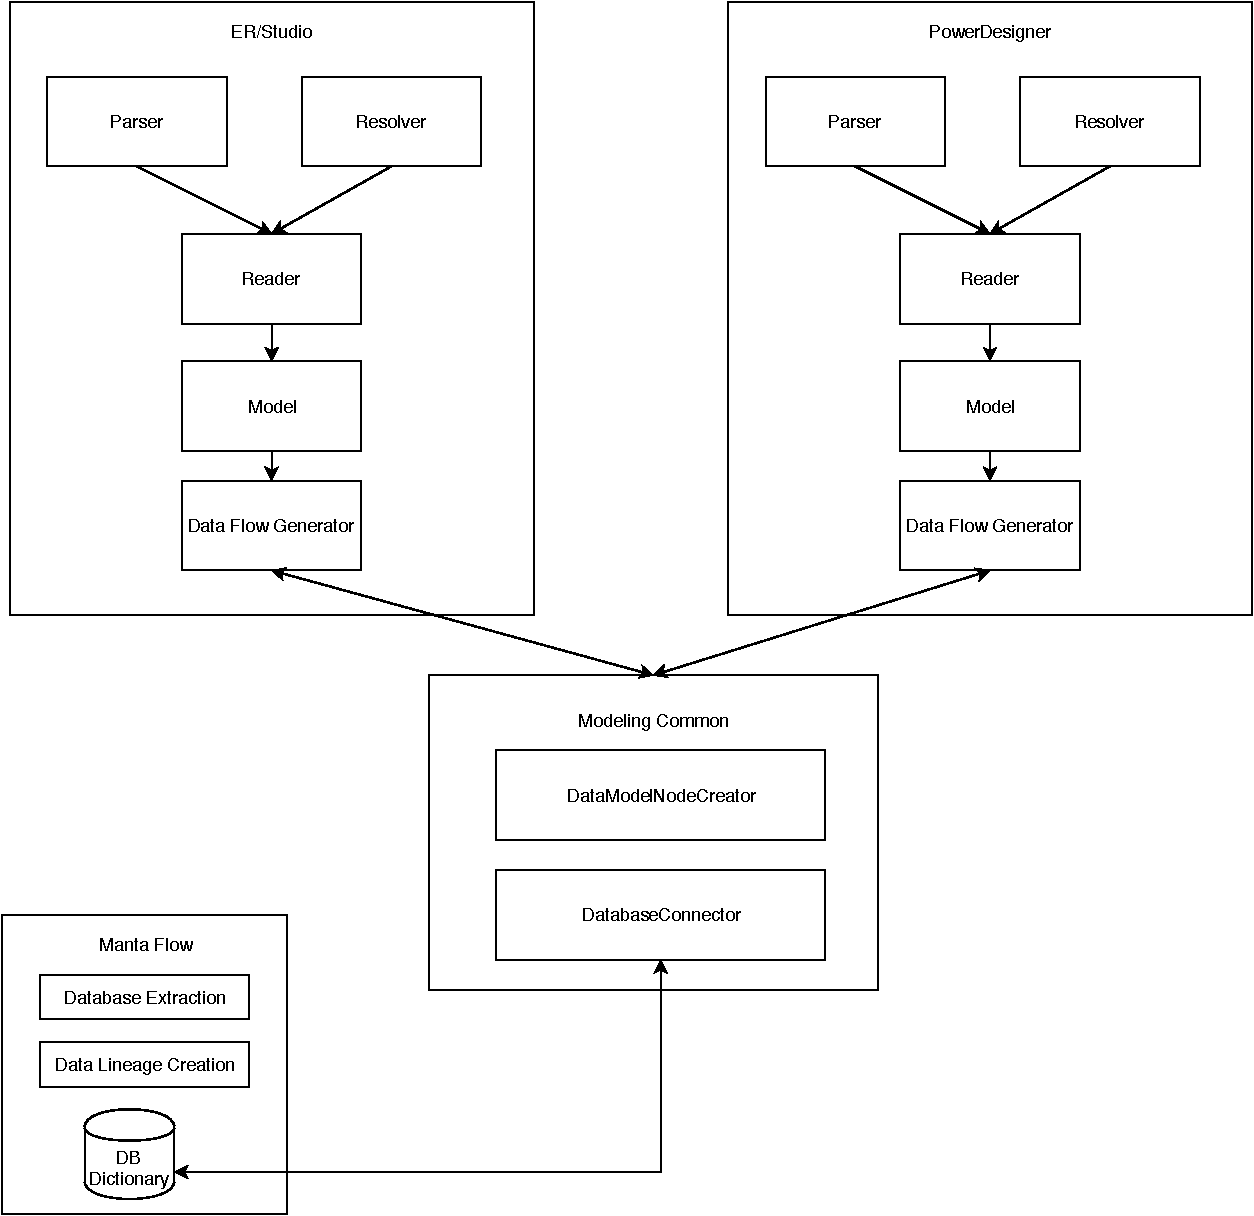
\includegraphics[height=14cm]{../img/SWArchitecture}
	\caption[Metadata Extractor Software Architecture]{A high level view on software architecture of Metadata Extractor}
	\label{SWArchitecture}
\end{figure}